\section{Continuous Random Variables}

A \emph{continuous random variable} is
analogous to the discrete case. Recall that
a probability is just a size of a set.
It's easy to find the size of a discrete set
because you can just count elements, but for
an uncountable set new methods are needed. Luckily
the intution for continuous random variables is
intuitive, it's still just the size of a set $A$
relative to $\Omega$.
\begin{figure}[h]
    \centering
    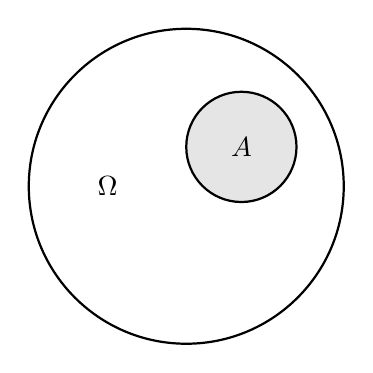
\begin{tikzpicture}[scale=1]
        \draw[thick] (0,0) circle (2cm);
        \node at (-1,0) {$\Omega$};
        \draw[thick, fill=gray!20] (0.7,0.5) circle (0.7cm);
        \node at (0.7,0.5) {$A$};
    \end{tikzpicture}
    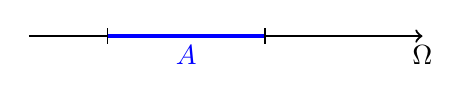
\begin{tikzpicture}[scale=1]
        \draw[thick,->] (0,0) -- (5,0);
        \node[below] at (5,0) {$\Omega$};
        \draw[very thick,blue] (1,0) -- (3,0);
        \node[below,blue] at (2,0) {$A$};
        \draw (1,0.1) -- (1,-0.1);
        \draw (3,0.1) -- (3,-0.1);
    \end{tikzpicture}
    \caption{Continuous random variables}
\end{figure}
Formally, if each event in A is equally likely, then
\begin{equation}
    P[\{x \in A\}] = \frac{\int_{A}dx}{|\Omega|}
\end{equation}
If we relax the assumption of equiprobability, then
more generally
\begin{equation}
    P[\{x\in A\}] = \int_{A} f_X(x) dx
\end{equation}
$f_X(x)$ is called the \emph{probability density function} (PDF).
It is analogous to the probability mass function.

Formally, a probability density function
is a mapping $f_X: \Omega \implies \Re$,
with the following properties:
\begin{itemize}
    \item Non-negativity: $f_X(x) \geq 0 \forall x \in \Omega$
    \item Unity: $\int_{\Omega} f_X(x)dx = 1$
    \item Measure of a set: $P[\{x \in A\}] = \int_{A}f_X(x) dx$
\end{itemize}

We can express a PDF in terms of a PMF
with a train of delta functions like so:
\begin{equation}
    f_X(x) = \sum_{x_k \in \Omega} p_X(x_k) \delta(x - x_k)
\end{equation}

We can also define the probability density
function as the derivative of the CDF, like so:
\begin{equation}
    f_X(x) = \frac{d}{dx}p(X \leq x)
\end{equation}

The expectation of a continuous random variable is
\begin{equation}
    E[X] = \int_{\Omega} xf_X(x)dx
\end{equation}

Properties of the expectation for continuous
random variables:
\begin{itemize}
    \item $E[aX] = aE[X]$
    \item $E[X+a] = E[X] + a$
    \item $E[aX+b] = aE[X] + b$
\end{itemize}

A random variable $X$ has an expectation
if it is absolutely integrable,
\begin{equation}
    E[|X|] = \int_{\Omega} |x|f_X(x)dx < \infty
\end{equation}

The variance of a continuous random variable
$X$ is
\begin{align}
    Var[X] & = E[(X-\mu)^2]                    \\
           & = \int_{\Omega} (x-\mu)^2f_X(x)dx \\
           & = E[X^2] - \mu^2
\end{align}

A continuous \emph{uniform random variable}
has a PDF of
\begin{equation}
    f_X(x) = \begin{cases}
        \frac{1}{b-a} & a \leq x \leq b \\
        0             & \text{else}
    \end{cases}
\end{equation}
We write
\begin{equation}
    X \sim Uniform(a,b)
\end{equation}
to mean that $X$ is drawn from a uniform
distribution on an interval $[a, b]$.
It has a CDF given by
\begin{equation}
    F_X(x) = \begin{cases}
        0               & x < a           \\
        \frac{x-a}{b-a} & a \leq x \leq b \\
        1               & x > b
    \end{cases}
\end{equation}
If $X \sim Uniform(a,b)$ then
\begin{align}
    E[X]   & = \frac{a + b}{2}      \\
    Var[X] & = \frac{(b - a)^2}{12}
\end{align}

A continuous \emph{exponential random variable}
has a PDF of
\begin{equation}
    f_X(x) = \begin{cases}
        \lambda e^{-\lambda x} & x \geq 0    \\
        0                      & \text{else}
    \end{cases}
\end{equation}
\marginnote{An exponential random variable
    is the interarrival time between two consecutive
    Poisson events}
We write
\begin{equation}
    X \sim Exponential(\lambda)
\end{equation}
to mean that $X$ is drawn from an
exponential distribution of parameter
$\lambda$. It has a CDF given by
\begin{equation}
    F_X(x) = 1 - e^{-\lambda x}
\end{equation}
If $X \sim Exponential(\lambda)$, then
\begin{align}
    E[X]   & = \frac{1}{\lambda}   \\
    Var[X] & = \frac{1}{\lambda^2}
\end{align}

A \emph{Gaussian random variable} is a
random variable $X$ such that its PDF
is
\begin{equation}
    f_X(x) = \frac{1}{\sqrt{2\pi \sigma^2}}\exp\left(-\frac{(x-\mu)^2}{2\sigma^2}\right)
\end{equation}
We write
\begin{equation}
    X \sim Gaussian(\mu, \sigma^2)
\end{equation}
or
\begin{equation}
    X \sim \mathcal{N}\left(\mu, \sigma^2\right)
\end{equation}
to mean that $X$ is drawn from a Gaussian
of parameter $(\mu, \sigma^2)$.
If $X \sim \mathcal{N}(\mu, \sigma^2)$, then
\begin{align}
    E[X]   & = \mu      \\
    Var[X] & = \sigma^2
\end{align}

The \emph{standard Gaussian} random variable has a
PDF given by
\begin{equation}
    f_X(x) = \frac{1}{\sqrt{2\pi}} e^{-\frac{x^2}{2}}
\end{equation}
The CDF of the standard Gaussian is defined
as the $\Phi$ function.
\begin{equation}
    \Phi(x) = \frac{1}{\sqrt{2\pi}}\int_{-\infty}^{\infty} e^{-\frac{t^2}{2}}dt
\end{equation}
The CDF of the standard Gaussian is related to the
\emph{error function}, which is defined as
\begin{equation}
    \text{erf}(x) = \frac{2}{\sqrt{\pi}} \int_{0}^{x} e^{-t^2} dt
\end{equation}
by the relation
\begin{equation}
    \Phi(x) = \frac{1}{2} \left(1 + \text{erf}\left(\frac{x}{\sqrt{2}}\right)\right)
\end{equation}
The CDF of an arbitrary Gaussian is related via
the transformation
\begin{equation}
    F_X(x) = \phi\left(\frac{x - \mu}{\sigma}\right)
\end{equation}
Let $X \sim \mathcal{N}(\mu, \sigma^2)$, then
\begin{itemize}
    \item $\Phi(y) = 1 -\Phi(-y)$
    \item $P[X\geq b] = 1 - \Phi(\frac{b-\mu}{\sigma})$
    \item $P[|X| \geq b] = 1 - \Phi(\frac{b-\mu}{\sigma}) + \Phi(\frac{-b-\mu}{\sigma})$
\end{itemize}

In addition to mean and variance, we introduce
two more useful quantities, \emph{skewness} and
\emph{kurtosis}.
\begin{align}
    E\left[X\right]                                   & = \mu      \\
    E\left[(X - \mu)^2\right]                         & = \sigma^2 \\
    E\left[\left(\frac{X-\mu}{\sigma}\right)^3\right] & = \gamma   \\
    E\left[\left(\frac{X-\mu}{\sigma}\right)^4\right] & = \kappa
\end{align}
\marginnote{\emph{Excess kurtosis} is defined
    as $\kappa - 3$}

Skewness measures the asymmetry of a
distribution. A Gaussian distribution has
skewness 0. Kurtosis measures how heavy-tailed
the distribution is. If the kurtosis is
positive, then the tails decay faster than a
Gaussian. If the kurtosis is negative, then
the distribution has a tail that
decays more slowly than a Gaussian.

The definition of a CDF is
\begin{equation}
    F_X(x) = P[X \leq x]
\end{equation}
\begin{figure}
    \centering
    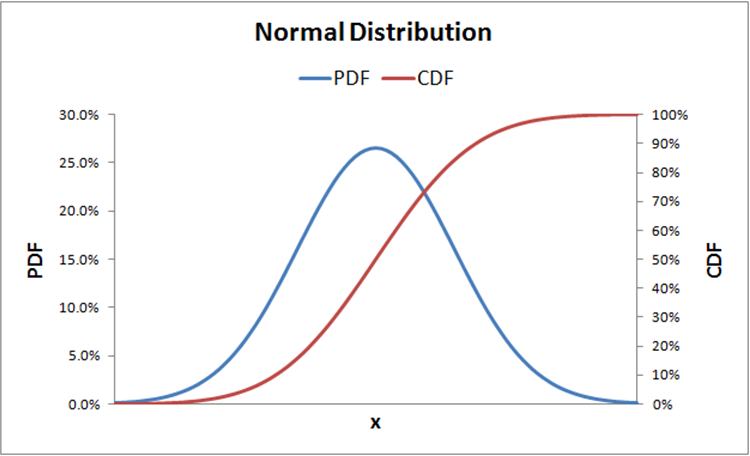
\includegraphics[scale=0.5]{images/normal_distribution_plot.png}
    \caption{PDF and CDF}
\end{figure}
Let $X$ be a continuous random variable. if the CDF
$F_X$ is continuous at any $a\leq x \leq b$, then
\begin{equation}
    P[a \leq X \leq b] = F_X(b) - F_X(a)
\end{equation}
A function $F_X(x)$ is said to be left
continuous if at $x=b$
\begin{equation}
    F_X(b) = \lim_{h\implies 0} F_X(b-h)
\end{equation}
and right continuous if
\begin{equation}
    F_X(b) = \lim_{h\implies 0} F_X(b+h)
\end{equation}
and continuous if $F_X(x)$ is both left
and right continuous.
All CDFs are right continuous.

For any random variable $X$, discrete or continuous,
\begin{equation}
    P[X=b] = \begin{cases}
        F_X(b) - F_X(b^-) & \text{if $F_X$ is discontinuous at $x=b$} \\
        0                 & \text{else}
    \end{cases}
\end{equation}

The PDf is the derivative of the CDF.
\begin{equation}
    f_X(x) = \frac{d}{dx} \int_{-\infty}^{x} f_X(t)dt
\end{equation}
provided $F_X$ is differentiable at $x$. If not, then
\begin{equation}
    f_X(x) = F_X(x) - \lim_{h\implies 0} F_X(x-h)
\end{equation}

Let $X$ be a continuous random variable with PDF
$f_X$. The median of $X$ is a point $c \in \Re$ such that
\begin{equation}
    \int_{-\infty}^{c} f_X(x) dx = \int_{c}^{\infty}f_X(x) dx
\end{equation}

Let $X$ be a continuous random variable. The mode is
the point $c$ such that $f_X(x)$ attains the maximum.
\begin{equation}
    x = \text{argmax}_{x \in \Omega} f_X(x)
\end{equation}

The mean $E[X]$ can be computed from
$F_X$ as
\begin{equation}
    E[X] = \int_{0}^{\infty} (1-F_X(t))dt
\end{equation}

Recall that joint distributions are
higher-dimensional PDFs, PMFs, or CDFs.
\begin{equation}
    f_{\textbf{X}}(\vec{x}) = f_{X_1, \dots, X_N}(x_1, \dots, x_n)
\end{equation}
Let $X$ and $Y$ be two continuous random variables.

The \emph{joint PDF} of $X$ and $Y$ is a function
$f_{X,Y}(x,y)$ that can be integrated to yield a probability
\begin{equation}
    P[A] = \int_{A} f_{X,Y}(x,y)dxdy
\end{equation}
for any event $A \subseteq \Omega_X \times \Omega_Y$.

The \emph{marginal PDF} is defined as
\begin{equation}
    f_X(x) = \int_{\Omega_Y} f_{X,Y}(x,y)dy
\end{equation}
and
\begin{equation}
    f_Y(y) = \int_{\Omega_X} f_{X,Y}(x,y)dx
\end{equation}

The \emph{marginal CDF is}
\begin{align}
    F_X(x) & = F_{X,Y}(x, \infty) \\
    F_Y(y) & = F_{X,Y}(\infty, y)
\end{align}

Let $F_{X,Y}(x,y)$ be the joint CDF of $X$ and $Y$.
Then the joint PDF can be obtained through
\begin{equation}
    f_{X,Y}(x,y) = \frac{\partial^2}{\partial_y\partial_x} F_{X,Y}(x,y)
\end{equation}

If two random variables are \emph{independent},
then
\begin{equation}
    p_{X,Y}(x,y) = p_X(x)p_Y(y)
\end{equation}
and
\begin{equation}
    f_{X,Y}(x,y) = f_X(x)f_Y(y)
\end{equation}

If a sequence of random variables
$X_1, \dots, X_N$ are independent,
then their joint PDF can be factorized.
\begin{equation}
    f_{X_1,\dots,X_N}(x_1,\dots,x_n) = \prod_{n=1}^{N}f_{X_n}(x)n
\end{equation}

A collection of random variables $X_1, \dots, X_N$ are called
\emph{independent and identically distributed} (i.i.d.) if
all are independent and have the same distribution, i.e.
$f_{X_1}(x) = \dots = f_{X_N}(x)$.

The \emph{joint expectation} is
\begin{equation}
    E[XY] = \int_{y\in \Omega_y}\int_{x\in \Omega_x} xy f_{X,Y}(x,y)dxdy
\end{equation}

For an arbitrary $g(X,Y)$,
\begin{equation}
    E[g(X,Y)] = \int_{y\in \Omega_y}\int_{x\in \Omega_x} g(x,y) f_{X,Y}(x,y)dxdy
\end{equation}

Recall
\begin{equation}
    \text{Cov}(X,Y) = E[XY] - E[X]E[Y]
\end{equation}
and now we also state that
\begin{equation}
    \text{Var}[X+Y] = \text{Var}[X] + 2\text{Cov}(X,Y) + \text{Var}[Y]
\end{equation}
We also state that covariance is zero, then so is the correlation.
However if the correlation is zero, the covariance is not necesarily zero.
\begin{equation}
    \text{Cov}(X,Y) = 0 \implies \text{Corr}(X,y) = 0
\end{equation}

If $X$ and $Y$ are independent, then
\begin{equation}
    E[XY] = E[X]E[Y]
\end{equation}
This implies that $X$ and $Y$ are
uncorrelated (i.e. $\text{Cov}(X,Y) = 0$),
but the converse is not true.

Let $X$ and $Y$ be two continuous random variables.
The \emph{conditional PDF} of $X$ given $Y$ is
\begin{equation}
    f_{X|Y}(x|y) = \frac{f_{X,Y}(x,y)}{f_Y(y)}
\end{equation}

Let $X$ and $Y$ be continuous random variables and
$A$ be an event. Then
\begin{equation}
    P[X \in A | Y=y] = \int_{A} f_{X|Y}(x|y)dx
\end{equation}
\begin{equation}
    P[X\in A] = \int_{\Omega_Y} P[X\in A|Y = y]f_Y(y)dy
\end{equation}

The \emph{conditional expectation} of $X$ given $Y=y$ is
\begin{equation}
    E[X|Y=y] = \int_{-\infty}^{\infty}xf_{X|Y}(x|y)dx
\end{equation}

The \emph{law of total expectation} is
\begin{equation}
    E[X] = \int_{-\infty}^{\infty} E[X|Y=y]f_Y(y)dy
\end{equation}
The theorem is sometimes also written
\begin{equation}
    E[X] = E_Y[E_{X|Y}[X|Y]]
\end{equation}